% Chapter Template

\chapter{Hyperbolic geometry} % Main chapter title

\label{Chapter1} % Change X to a consecutive number; for referencing this chapter elsewhere, use \ref{ChapterX}
\thispagestyle{empty}
%----------------------------------------------------------------------------------------
%	SECTION 1
%----------------------------------------------------------------------------------------

\section{Iwasawa decomposition}

\begin{impTeo}{Iwasawa (real) decomposition}{iwasawa}
For every matrix $M\in\SL_{2}\R$ there exist real matrices $K,A,N$ such that $M=KAN$ and 
\begin{align*}
K\in\mathfrak{K}&=\SO_{2}\R\\
A\in\mathfrak{A}&=\left\{
\Smallmatrix{a&0\\0&a^{-1}}\,\colon a\in\R_{>0}
\right\}\\
N\in\mathfrak{N}&=\left\{
\Smallmatrix{1&b\\0&a1}\,\colon b\in\R
\right\}
\end{align*}
\end{impTeo}

The Iwasawa decomposition of a matrix $M$ ultimately let you see it's action as the composition of three fundamental subgroups of $\GL_{2}\R$. This decomposition naturally implies the same decomposition using the projective linear group $\PSL_{2}\R$ instead of $\SL_{2}\R$. This feature is of particular interest for us because, as we shall se, $\PSL_{2}\R$ is the isometry group of the hyperbolic plane.


\section{Hyperbolic models: upper-half plane and disk}

\label{sec:hyp_plane}
\subsection{Hyperbolic plane}

We will now introduce the hyperbolic plane and some of its fundamental charateristics. A good complete reference for hyperbolic geometry is \cite{Katok:groups}. As starting point, we will consider the \textbf{upper-half plane} model, i.e. the set 
\[
\Hilb = \R\times \R_{>0} = \left\{z\in\mathbb{C}\colon \Im(z)>0\right\}
\]
with the metric tensor given by 
\[
g=\frac{1}{y^{2}}(\dd x^{2}+\dd y^{2}).
\]
The couple $(\Hilb,g)$ gives us a Riemannian manifold, as the metric tensor $g$ is positive definined. Moreover we can compute the Gaussian curvature $\kappa$ of this model, using the fact that 
\[
\kappa=\frac{1}{2}\bar{R}
\]
where $\bar{R}$ is the Ricci scalar. The component of the Ricci tensor are obtained by contracting the indices of Riemann tensor $R\indices{_{abcd}}$ with the inverse metric tensor $g^{ac}$. Riemann tensor has $16$ components, but with easy calculations one ends up with 
\[
R\indices{^{1}_{212}}=-R\indices{^{1}_{221}}=R\indices{^{2}_{121}}=-R\indices{^{2}_{112}}=y^{-2}
\]
and all the other components vanish. Hence 
\[
R_{1212}=R_{2121}=-y^{-4}\text{ and }R_{1221}=R_{2112}=y^{-4}.
\]
It can be seen that, using Einstein notation, it holds
\[
R_{cadb}=y^{-4}(1-\delta_{ab}-\delta_{cd})(1-\delta_{ac}),\; g^{ab}=y^{2}\delta^{ab}
\]
Finally,
\begin{align*}
R_{ab} &= g^{cd}R_{cadb}=y^{2}\delta^{cd}y^{-4}(1-\delta_{ab}-\delta_{cd})(1-\delta_{ac})\\
& = y^{-2}(\delta^{cd}-\delta^{cd}\delta_{ab}-\delta^{cd}\delta_{cd}-\delta^{cd}\delta_{ac}+\delta^{cd}\delta_{ab}\delta_{ac}+\delta^{cd}\delta_{cd}\delta_{ac}) \\
& = y^{-2}(2-2\delta_{ab}-2-1+\delta_{ab}+1)=-y^{-2}\delta_{ab}
\end{align*}
and then
\[
R=g^{ab}R_{ab}=-2
\]
which yields $\kappa=-1$. This justify the \virg{hyperbolic} adjective, the upper-half plane model is an example of a manifold with constant negative curvature. As we shall se, this greatly modifies the geometrical properties that we are used to.

We will consider the tangent bundle $T\Hilb$ of the hyperbolic plane and the norm of a vector $\tau$ in the tangent space $T_{z}$ is given by
\[
\norm{\tau}_{z}=\sqrt{\pscl{\tau}{\tau}_{g,z}}=\frac{\abs{\tau}}{\Im(z)}.
\]
The unit tangent bundle is given by
\[
T^{1}\Hilb\coloneqq\left\{
(z,\tau)\in T\Hilb\colon \abs{\tau}=\Im(z)
\right\}
\]
of tangent vectors with lentgh 1. In this context, the (hyperbolic distance) between two points $z,w\in\Hilb$ can be defined as 
\[
d\colon\Hilb\times\Hilb\to[0,+\infty],\quad d(z,w)=\inf_{\gamma} L(\gamma)
\]
where the infimum runs over all curves $\gamma\colon[0,1]\to\Hilb$ such that $\gamma(0)=z,\gamma(1)=w$, and the length of the curve is defined as
\[
L(\gamma)\coloneqq\int_{0}^{1}\norm{\gamma'(t)}_{z}\dd t=\int_{0}^{1}\norm{\gamma'(t)}_{z}\frac{\dd t}{\Im(\gamma(t))}.
\]

It's interesting to determin and analyze the isometry group of $(\Hilb,g)$ with respect to the hyperbolic metric. More precisely, the set $\Isom(\Hilb)$ is the set of smooth maps $\vphi\colon\Hilb\to\Hilb$ that are metric-preserving, i.e. 
\[
\norm{\Diff\vphi(\tau)}_{\vphi(z)}=\norm{\tau}_{z},\quad\forall(z,\tau)\in TM
\]
The group $\PSL_{2}\R$ naturally acts on the extended hyperbolic plane $\hat{\Hilb}=\Hilb\cup\{\infty\}$ via \emph{M{\" o}bius transformations}. For any $A=\SmallQmatrix{a&b\\c&d}\in\PSL_{2}\R$, we get 
\[
A\ast z=\frac{az+b}{cz+d}
\]
if $z\in\Hilb$ and $A\ast\infty=a/c$, where $a/c=\infty$ if $c=0$. The action is well defined, as, if $\Im(z)>0$, than 
\[
\Im(A\ast z)=\frac{\Im(z)}{\abs{cz+d}^{2}}>0.
\]
For the sake of brevity, we will use $A(z)$ instead of $A\ast z$. This action generalize to an action on the unit tangent bundle $T^{1}M$ given by
\[
A\ast(z,\tau)=(A(z),\Diff A_{\ast}\tau).
\]
We will denote the action of $A$ on tangent vector $\tau$ at point $z$ with $\Diff_{z} A\tau$.\\

The action on $T^{1}M$ is faithfully and moreover is transitive. For this, it's sufficient to show that any element $(z,\tau)$ is in the $\PSL_{2}\R$-orbit of $(\imi,\imi)$. We have that
\[
\Qmatrix{1&x\\0&1}\Qmatrix{y^{1/2}&0\\0&y^{-1/2}}\imi=x+\imi y=z
\] 
and so, if $B=\SmallQmatrix{1&x\\0&1}\SmallQmatrix{y^{1/2}&0\\0&y^{-1/2}}=\SmallQmatrix{y^{1/2}&xy^{-1/2}\\0&y^{-1/2}}$, we have that $B^{-1}(z)=\imi$. In particular, the action of $B^{-1}$ on the tangent vector $\tau$ is the identity. Hence $B^{-1}\ast(z,\tau)=(\imi,\tau)$. Via straightforward computation, it can be shown that the subgroup $\SO_{2}\R$ is the stabilizer of point $\imi$ and acts as a rotation on the tangent vector $\tau$. In particular, if $\tau=e^{\imi\theta}$, let $\alpha=\frac{1}{2}\left(\frac{\pi}{2}-\theta\right)$. Then
\begin{align*}
\Diff_{\imi}\Qmatrix{\cos\alpha&-\sin\alpha\\ \sin\alpha&\cos\alpha}\imi&=\frac{\imi}{(\cos\alpha+\imi\sin\alpha)^{2}}=\imi \e^{-2\imi\alpha}\\
&=\imi \e^{-\imi\pi2}\e^{\imi\theta}=\imi(\imi)\tau=\tau
\end{align*}
and hence, if
\begin{equation}
\label{eq:main_matrix}
A=B\Qmatrix{\cos\alpha&-\sin\alpha\\\sin\alpha&\cos\alpha}=\Qmatrix{1&x\\0&1}\Qmatrix{y^{1/2}&0\\0&y^{-1/2}}\Qmatrix{\cos\alpha&-\sin\alpha\\\sin\alpha&\cos\alpha}
\end{equation}
we get that $A\ast(\imi,\imi)=(z,\tau)$. In particular this is the only matrix $A\in\PSL_{2}\R$ such that $A\ast(\imi,\imi)=(z,\tau)$. Hence, we have following.
\begin{nlem}
\label{lem:t1h_psl2_identification}
$T^{1}\Hilb$ and $\PSL_{2}\R$ are homeomorphic.
\end{nlem}
\begin{prf}
The action of matrix \eqref{eq:main_matrix} defines the desired homeomorphism.
\end{prf}

The group $\PSL_{2}\R$ coincides with the group $\Isom\Hilb$, as stated by the following theorem.

\begin{nteo}
\label{teo:area_volume_forms_invariants_isometries}
The left action of $\PSL_{2}\R$ on $T\Hilb$ it's transitive and preserves the area and volume forms
\[
\dd A=\frac{\dd x\wedge\dd y}{y^{2}},\quad\dd V=\frac{\dd x\wedge\dd y\wedge\dd\theta}{y^{2}}.
\]
In particular, the action of $A\in\PSL_{2}\R$ is an isometry.
\end{nteo}


At this point, it's crucial to establish some characterization of the geodesics, i.e. curves of minimal length connecting two given points. It can be shown the following result.

\begin{nprop}
\label{prop:geod_hyp}
The geodesics are the vertical lines and the semi-circles centred on the real axis.
\end{nprop}
\begin{prf}
Let $z,w\in\Hilb$. Let's assume first that $z=a\imi$ and $w=b\imi$, with $b>a>0$. Let $\eta(t)=t\imi$ with $t\in[a,b]$. Then 
\[
L(\eta)=\int_{a}^{b}\norm{\eta'(t)}_{\Hilb}\dd t=\int_{a}^{b}\frac{\abs{\imi}}{t}\dd t=\ln(b/a).
\]
Moreover, for a generic path 
\[
\gamma\colon[a,b]\to\Hilb,\,\gamma(t)=x(t)+y(t)\imi
\] 
such that $\gamma(a)=z$ and $\gamma(b)=w$, we have that
\[
L(\gamma)=\int_{a}^{b}\frac{\sqrt{x'(t)^{2}+y'(t)^{2}}}{y(t)}\geq\int_{a}^{b}\frac{\abs{y'(t)}}{y(t)}\dd t\geq\int_{a}^{b}\frac{\dd y}{y}=\ln(b/a)
\]
and hence $\ln(b/a)$ is the hyperbolic length of the segment of the $y$-axis joining $a\imi$ and $b\imi$. As this is valid for any point of the imaginary axis, we deduce that this axis is a geodesic.\\
Now, for two arbitrary points $z,w\in\Hilb$ it's sufficient to proceed as follows. Let $\mathcal{G}$ the unique vertical line or circle centered on the real axis passing through these two points. If $\mathcal{G}$ is a vertical axis $a+t\imi$, the matrix $\Qmatrix{1&-a\\0&1}$ shifts this line to the imaginary axis; if otherwise $\mathcal{G}$ is a semicircle with endpoints $a,b$ on the real axis, the matrix $\Qmatrix{0&-1\\1&-b}$ maps $\mathcal{G}$ to the imaginary axis. In both cases, with an element $A\in\PSL_{2}\R$ we can map $z,w$ on the imaginary axis and conclude as before. As $\PSL_{2}\R$ transformations are isometries, this shows what desired.
\end{prf}

Having described the hyperbolic geodesics, it would be useful to have a closed formula for the (hyperbolic) distance of two points. This is established by the following lemma.
\begin{nlem}
\label{lem:hyp_distance_formula}
For $z,w\in\Hilb$, we have 
\[
\cosh d_{\Hilb}(z,w)=1+\frac{\abs{z-w}^{2}}{2\Im(z)\Im(w)}.
\]
\end{nlem}
\begin{prf}
Let's assume first that $z=a\imi$ and $w=b\imi$, with $b>a>0$. Then 
\[
\cosh d_{\Hilb}(a\imi,b\imi)=\cosh\ln(b/a)=\frac{1}{2}\left(\frac{b}{a}+\frac{a}{b}\right)
\]
and 
\[
1+\frac{\abs{z-w}^{2}}{2\Im(z)\Im(w)}=\frac{a^{2}+b^{2}}{2ab}.
\]
Now, it's sufficient to show that the right hand side of the equality is invariant under the action of $A\in\PSL_{2}\R$ to conclude as in the previous result. This is left as exercise.
\end{prf}


Having the isometry group $\PSL_{2}\R$ of the upper-half plane model at hand and a characterization of geodesics, it's now possible to briefly describe the actions of an arbitrarly element $A\in\PSL_{2}\R$. In this regard, it's helpful to introduce another model of the hyperbolic plane, namely Poincaré's disk model $\Disk$, which is the data of $(\Disk,\Dmetr)$
\[
\Disk=\left\{
z\in\mathbb{C}\colon\,\abs{z}<1
\right\},\quad \Dmetr=\frac{4}{(1-\abs{z}^{2})^{2}}(\dd x^{2}+\dd y^{2})
\]
This model is totally equivalent with the upper-half plane model $\Hilb$ as they can be isometrically equivalent via the map 
\[
\Cayley\colon\Hilb\to\Disk,\quad\Cayley(z)\coloneqq\frac{\imi z+1}{z+\imi}
\]
induced, with abuse of notation, by the matrix $\Cayley=\frac{1}{\sqrt{2}}\SmallQmatrix{\imi&1\\1&\imi}$.\\

To see this, if $w=C(z)$ and $z=x+\imi y$ with $y>0$, then
\begin{align*}
\abs{w}^{2}&=\abs{\frac{\imi z+1}{z+\imi}}^{2}=\frac{\imi z+1}{z+\imi}\overline{\frac{\imi z+1}{z+\imi}}\\
&=\frac{x^{2}+y^{2}+1-2y}{x^{2}+y^{2}+1+2y}<1.
\end{align*}
Moreover, if $\tau_{1},\tau_{2}$ are tangent vectors at $z$, then corrispondent tangent vectors $v_{i}=\Diff\Cayley \tau_{i}$ at $w$ are given by
\[
v_{i}=\frac{\tau_{i}}{(z-\imi)^{2}}
\]
and with easy computation one can show that $\Hmetr(\tau_{1},\tau_{2})=\Dmetr(v_{1},v_{2})$.

This model can be more appropriate to describe some actions, as it's \virg{compact} and more symmetrical. In this model the geodesics are of two kind:
\begin{compactitem}
\item if $z,w\in\Disk$ are collinear with the origin $0$, then the geodesic is the only diameter passing through $z,w$;
\item otherwise, the geodesic connecting $z,w$ is the only circle passing through $z,w$ which is perpendicular\footnote{There is a nice geometrical construction for this: let $w^{\ast}$ be the point obtained inverting the point $w$ respect to the circle $\abs{z}=1$; the desired circle is the circle passing through $z,w,w^{\ast}$.} to $\partial\Disk$;
\end{compactitem}

\subsection{Hyperbolic isometries}

\label{subsec:hyp_isom}

As each element $A\in\PSL_{2}\R$ has determinat $1$, their action is determined by $\tr A$ (\textsc{wlog} we can assume $\tr A\geq0$, as $A$ is considered up to multiplication by $\pm I$). There are three cases:
\begin{compactitem}
\item $\tr A>2$, hyperbolic matrices;
\item $\tr A=2$, parabolic matrices;
\item $\tr A<2$, elliptic matrices.
\end{compactitem} 

Let's see briefly what their action is .\\[2mm]
\boldsf{Hyperbolic matrices}: $\tr A>2$\\
In this case, the eigenvalues are given by
\[
\lambda=\lambda_{1}=\frac{\tr A+\sqrt{\Delta}}{2}>1>\frac{\tr A-\sqrt{\Delta}}{2}=\lambda_{2}=\lambda^{-1},
\]
and are both real. If $v_{1},v_{2}$ are the two eigenvectors corrisponding respectivly to $\lambda_{1,2}$, matrix $A$ can be diagonalized by matrix $E=(v_{1}|v_{2})$, getting
\[
AE=E\Qmatrix{\lambda&\\&\lambda^{-1}}.
\]
Matrix $A$ acts on the plane $E\Hilb$ \virg{as} the matrix $D=\Smallmatrix{\lambda&\\&\lambda^{-1}}$ acts on $\Hilb$. In this case, the action is given explicity by $D(z)=\lambda^{2}z$ and this action is an (euclidian) homotety with center $0$ and factor $\lambda^{2}$. In particular, every points is attract to $\infty$ or to $0$ (depending whatever $\lambda\lessgtr1$).\\
For this reason, matrix $A$ it's a (hyperbolic) dilatation, of center $E\ast0$, factor $\lambda^{2}$ and direction $E\ast\infty$.%\\[2mm]

\begin{figure}[H]
\centering
  %
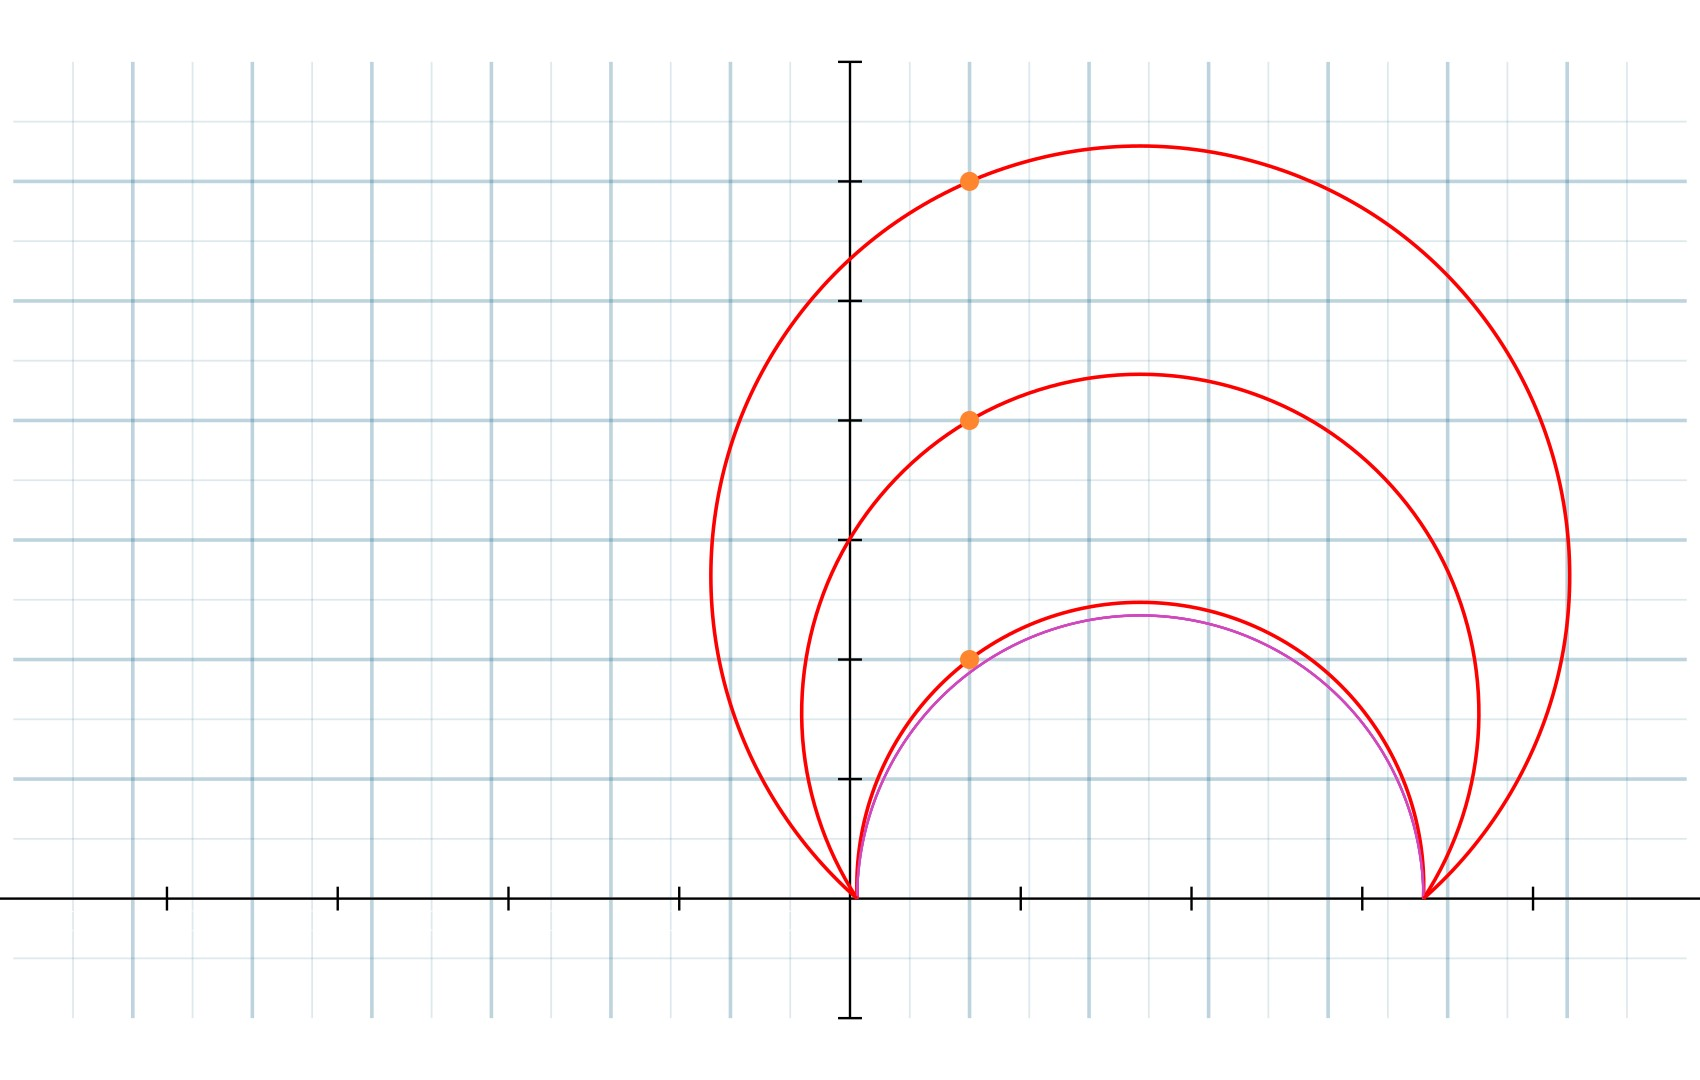
\includegraphics[scale=0.2,angle=0]{hyp_actions_hyp.jpg}
  \noindent\\
  \decoRule
  \caption{Action of an hyperbolic matrix on three point. In purple the \emph{axis}, see the end of this section.}
  \label{fig:hyp_action_hyp}
\end{figure}

\boldsf{Parabolic matrices}: $\tr A=2$\\
In this case the two eigenvalues are $\lambda_{1,2}=\lambda=1$. The matrix $A$ cannot be diagonalized, but it's similar to a matrix $D=\SmallQmatrix{1&T\\&1}$. In fact, fixed an eigenvector $v$ of $A$ for the eigenvalue $1$, this can form a basis for $\R^{2}$ with another indipendent vector $v'$. Moreover, re-scaling vector $v'$, we can suppose that $E=(v|v')$ has determinant $1$. Hence
\[
AE=E\Qmatrix{1&T\\&1}.
\]
As before, $A$ acts on the plane $E\Hilb$ \virg{as} the matrix $D=\Smallmatrix{\lambda&\\&\lambda^{-1}}$ acts on $\Hilb$. The action of $D$ is $D\ast z=z+T$, which is a horizontal translation with fixed point $\infty$. In particular, the orbits induced by $D$ can be considered as cirles of infinity ray with center at $\infty$. With this point of view, it's easy to describe the action of $A$: it's action will be a hyperbolic translation along circles which are tangets with line $\R\cup\{\infty\}$ at point $E\ast\infty$.%\\[2mm]
\begin{figure}[H]
\centering
  %
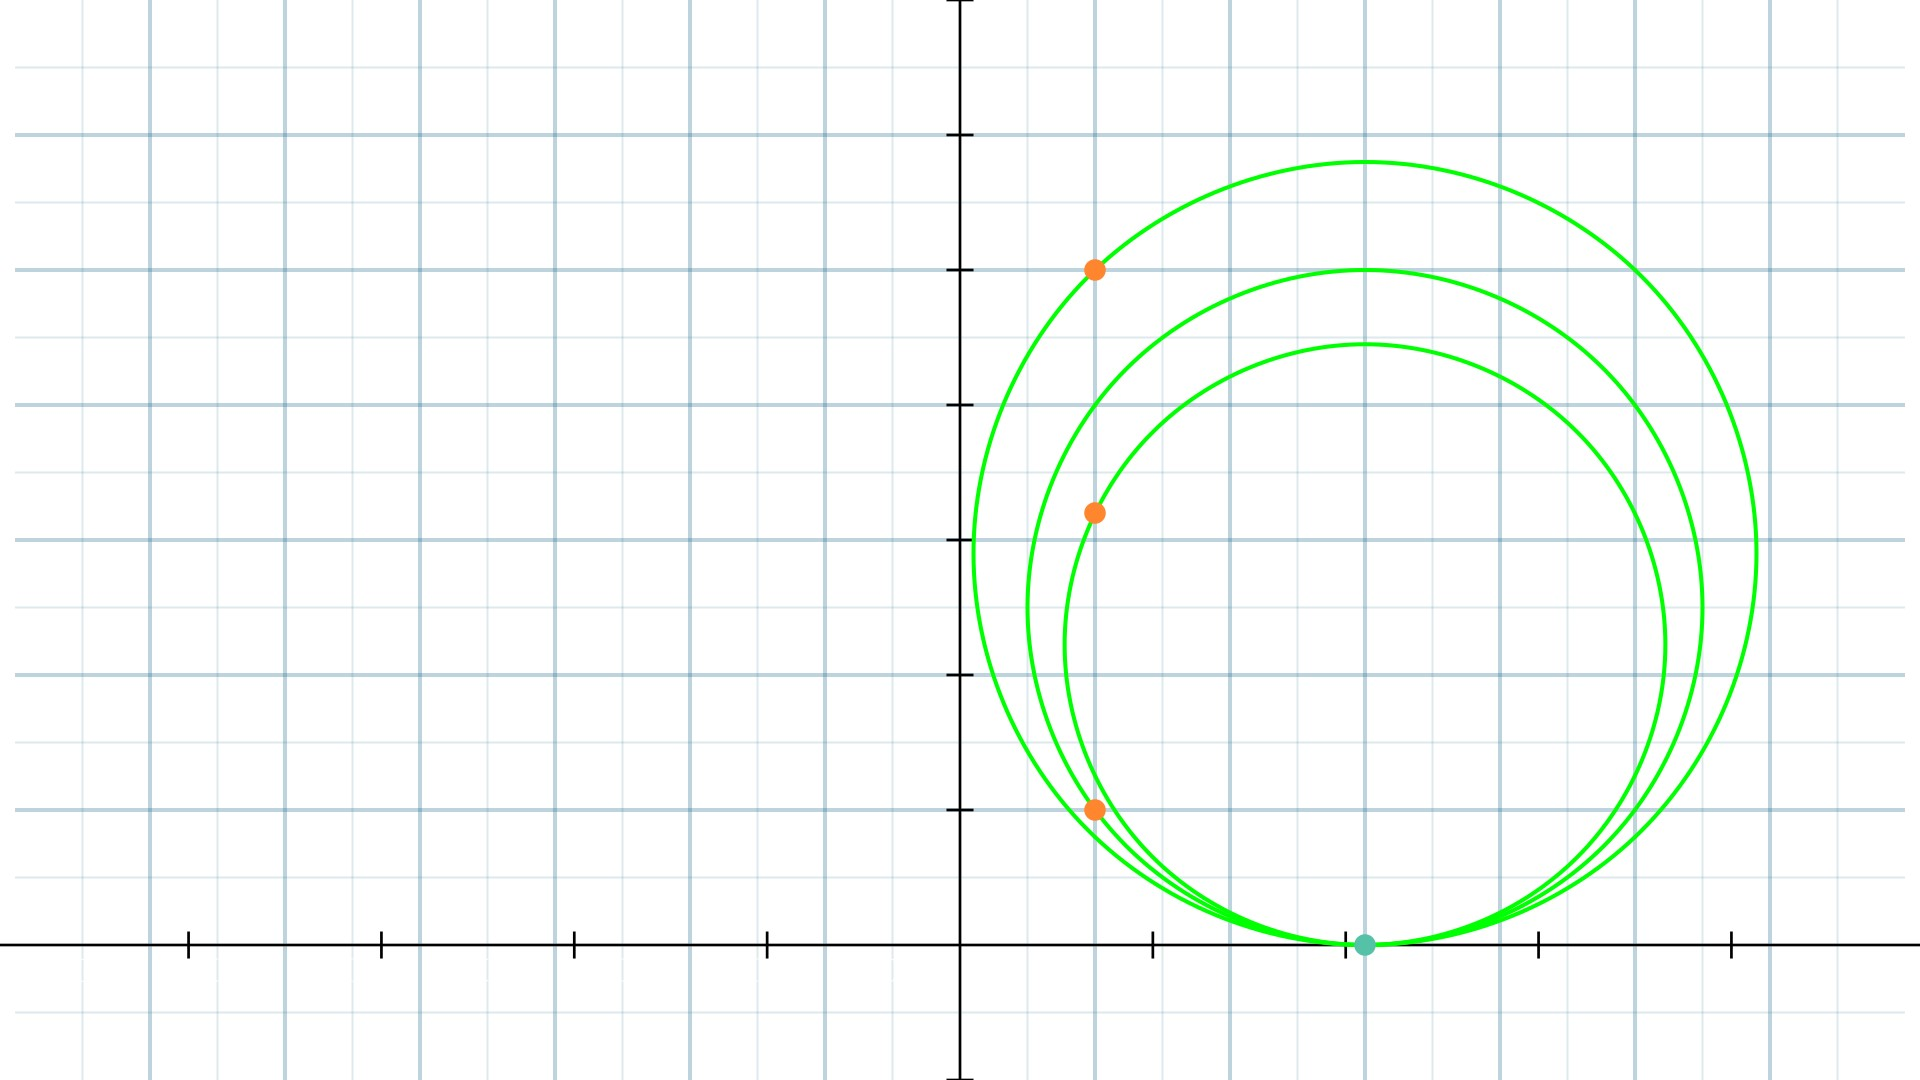
\includegraphics[scale=0.2,angle=0]{hyp_actions_parab.jpg}
  \noindent\\
  \decoRule
  \caption{Action of a parabolic matrix on three point.}
  \label{fig:hyp_action_parab}
\end{figure}


\boldsf{Elliptic matrices}: $0<\tr A<2$\\

In this case the eigenvalues are complex conjugated $\lambda=\lambda_{1}=\bar{\lambda}_{2}$ of modulus $1$ ($\lambda=e^{\imi\theta}$). Let $v$ the eigenvector corrisponding to the eigenvalue $\e^{\imi\theta}$, so that $\bar{v}$ is the eigenvector for $\e^{-\imi\theta}$. Let $E=(v+\bar{v},\imi(v-\bar{v}))$. Scaling $E$, we can make $\abs{\det T}=1$. 
\begin{figure}[H]
\centering
  %
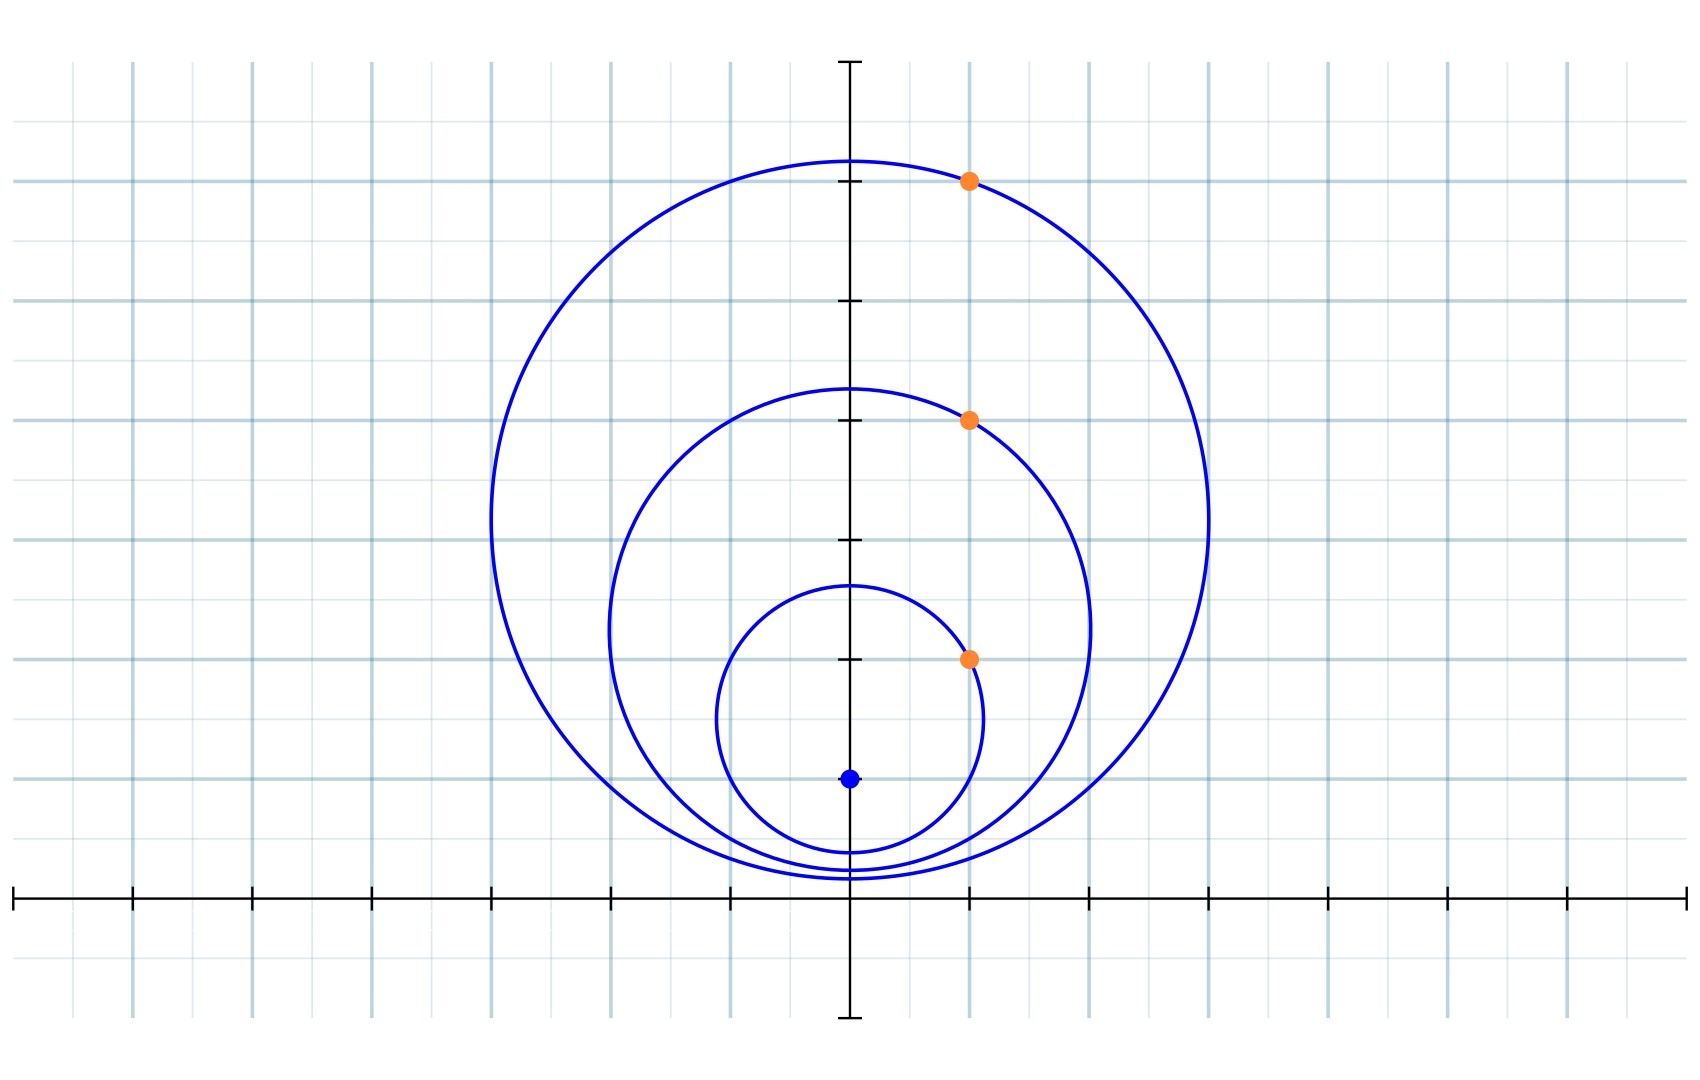
\includegraphics[scale=0.2,angle=0]{hyp_actions_ell.jpg}
  \noindent\\
  \decoRule
  \caption{Action of an elliptic matrix on three point.}
  \label{fig:hyp_action_ell}
\end{figure}
Let's assume $\det E=1$ (the other case is totally analogue). In this case,
\[
AE=E\Qmatrix{
\cos\theta&-\sin\theta\\\sin\theta&\cos\theta
}=ER
\]
$R$ fixes the point $\imi$. The action of $R$ can better visualized in Poincaré's disk model $\Disk$: the matrix $\Cayley$ sends $\imi$ in $0$ and the corrisponding matrix is given by
\[
\Cayley R\Cayley^{-1}=\Qmatrix{\e^{-\imi\theta}&\\&\e^{\imi\theta}}
\] 
and so the action on $\Disk$ is given by $z\mapsto\e^{-2\imi\theta}z$, which is exactly a rotation of angle $2\theta$ clockwise. In conclustion, the action of $A$ on $E\Hilb$ is given by hyperbolic rotations around the (unique) fixed point of $A$ in $\Hilb$.\\[2mm]

We could ask ourselves if any action of these matrices could send a geodesic into itself. In this sense, let's recall Iwasawa decomposition \ref{impTeo:iwasawa}: the action of a matrix is decomposed into the product $KAN$. Hence, given a matrix $KAN=M\in\PSL_{2}\R$, it's sufficient to check if there is an invariant geodesic whene $M$ is in one of three subgroups of Iwasawa decomposition.\\
If $M\in\PSO_{2}\R$, then $M$ it's a (hyperbolic) rotation around $\imi$ and then there is no invariant geodesic. In the same way, even if $M=\SmallQmatrix{1&x\\0&1}$ there are no invariant geodesics, as $M$ is an horizontal translation.\\
Diagonal matrices $A_{t}=\SmallQmatrix{\exp(t/2)&0\\0&\exp(-t/2)}$ instead send the $0-\infty$ geodesic into itself (and $0,\infty$ are fixed points for $A_{t}$). In general, an hyperbolic matrix $M$ with $\abs{\tr M}>2$ is conjugate to a matrix $A_{t}$ and so the geodesic connecting the two (real) fixed points of $M$ is invariant under the action of $M$.

It's possible to give an explicit description of this geodesic. Let $M=\SmallQmatrix{a&b\\c&d}$, then the fixed points are given by
\[
z_{1,2}=\frac{-(d-a\pm\sqrt{(d-a)^{2}+4cb})}{2c}=-\frac{d-a}{2c}\pm\frac{\sqrt{(d+a)^{2}-4}}{2c}
\]
and so the desired geodesic is the semicircle of center $z_{C}=-(d-a)/2c$ and radius $r=\sqrt{(d+a)^{2}-4}/(2\abs{c})$. So the equation of the geodesic is 
\begin{equation}
\label{eq:invar_geodes_hyperb}
\abs{z-z_{C}}^{2}=r^{2}\;\Leftrightarrow\;c\abs{z}^{2}-(d-a)\Re(z)-b=0
\end{equation}

If $c=0$, then the invariant geodesic is vertical, the details are left. In general, such an invariant geodesic is called \emph{\textbf{axis}} of hyperbolic matrix $M$.




\subsection{Hyperbolic surfaces and fuchsian groups}

\label{subsec:hyp_surfc}

The starting point to construct hyperbolic surfaces is to consider the analogue of euclidian lattice in this hyperbolic contest, i.e. fuchsian groups. The following result defines a fuchsian group.

\begin{nteo}
\label{teo:fuchs_theom_def}
Let $\Gamma$ be a $\PSL_{2}\R$ subgroup. The following are equivalent:
\begin{compactitem}
\item The action of $\Gamma$ on $\Hilb$ is properly discontinuos;
\item Each $\Gamma$-orbit on $\Hilb$ is discrete and each point has finite stabilizer;
\item $\Gamma$ is discrete with respect to $\PSL_{2}\R$ topology.
\end{compactitem}
\end{nteo}


\begin{defin}[Fuchsian group]
\label{def:fucs_def}
A subgroup $\Gamma$ of $\PSL_{2}\R=\Isom\Hilb$ that satisfies one of theorem \ref{teo:fuchs_theom_def} conditions is called \emph{fuchsian group}.
\end{defin}

We can get an \underline{hyperbolic surface} by considering the quotient $\Gamma\setminus\Hilb$. In this way, $M$ it's not necessarily a Riemann surface; in fact, if $\Gamma$ contains some elliptic points then $M$ it's an object called \emph{orbifold}. In general, we will assume that $\Gamma$ does not have any elliptic elements, with the important exceptions of triangular groups and the modular surface, see METTI SEZIONE più avanti. The following is essential to visualize the action of $\Gamma$.

\begin{defin}[Fundamental domain]
\label{def:fund_domain}
Let $\Gamma$ be a fuchsian group and let $\mu$ be the hyperbolic area form. Then $D\subset\Hilb$ is a fundamental domain for $\Gamma$ if 
\begin{compactitem}
\item $\bigcup_{\gamma\in \Gamma}\gamma\bar{D}=\Hilb$;
\item $\forall\gamma\neq1$, we have that $\mu(D\cap\gamma[D])=0$; if $D^{\mathrm{o}}\cap\gamma[D^{\mathrm{o}}]=\emptyset$, the fundamental domain is proper. 
\end{compactitem} 
\end{defin}

It can be shown that, if $D_{1},D_{2}$ are two fundamental domains of $\Gamma$ of finite area, then $\mu(D_{1})=\mu(D_{2})$. A special construction for a fundamental domain is given by Dirichlet.

\begin{defin}[Hyperbolic perpendicular bisector]
The \emph{perpendicular bisector} of a geodesic segment $[z,w]$ is the unique geodesic through the midpoint of $[z,w]$ and orthogonal to $[z,w]$.
\end{defin}

The idea of Dirichlet is to consider the set
\[
D=D_{p}(\Gamma)=\left\{
z\in\Hilb\colon d(z,p)<d(z,\gamma p)\;\forall\gamma\in\Gamma\setminus\{e\}
\right\}
\]
which is the intersection of hyperbolic half-planes 
\[
H_{p}(\gamma)=\left\{
z\in\Hilb\colon d(z,p)\leq d(p,\gamma z)
\right\}
\]
delimited by perpendicular bisector. It can be proved (\cite{Katok:groups}) that a Dirichlet domain is indeed a fundamental domain. Let's now consider some examples.

\begin{nese}[Triangular groups]
Consider an hyperbolic triangle with angles $\pi/a,\pi/b,\pi/c$. In particular it must hold
\[
\frac{1}{a}+\frac{1}{b}+\frac{1}{c}<1
\]
If $a,b,c$ are all integers (even $\infty$), then the group generated by reflections around the three sides of the triangle is a fuchsian group. It's denoted with $\triang^{\pm}(a,b,c)$. The group $\triang(a,b,c)$, instead, is the subgroup of index $2$ of $\triang^{\pm}(a,b,c)$ with transformations that preserver the orientation. In a more abstract way, a representation of an orientation-preserving triangle group is given by
\[
\triang(a,b,c)=\spn{
g_{a},g_{b},g_{c}\colon g_{a}^{a}=g_{b}^{b}=g_{c}^{c}=g_{a}g_{b}g_{c}=e
}.
\]
\end{nese}

There is a standard way to construct a triangular group with given integers $a,b,c$, by Petersson and recently revised by Voight (\cite{Voight:triang}, \cite{Peter:triang}). For $\N\ni t\geq 2$ let 
\[
\zeta_{t}=\e^{\frac{2\pi\imi}{t}},\quad \lambda_{t}=2\Re(\zeta_{t}),\quad \mu_{t}=2\Im(\zeta_{t}). 
\]
If $t=\infty$, then $\zeta_{\infty}=1$. Then, an immersion of $\triang^{\pm}(a,b,c)$ in $\PSL_{2}$ is given by $g_{a}\mapsto M_{a}, g_{b}\mapsto M_{b}$ and $g_{c}\mapsto M_{c}=-M_{b}^{-1}M_{a}^{-1}$ where 
\[
M_{a}=\frac{1}{2}\Qmatrix{\lambda_{2a}&\mu_{2a}\\-\mu_{2a}&\lambda_{2a}},\quad
M_{b}=\frac{1}{2}\Qmatrix{\lambda_{2b}&t\mu_{2c}\\-\mu_{2c}/t&\lambda_{2b}},
\]
with $t=c+\sqrt{c^{2}-1}, c=\frac{\lambda_{2a}\lambda_{2b}+2\lambda_{2c}}{\mu_{2a}\mu_{2b}}$. In particular, we have
\[
M_{a}^{a}=M_{b}^{b}=M_{c}^{c}=I.
\]
TO BE ADDED SOME FIGURES

\begin{nese}[Modular surface]
\label{ese:modular_surface}
The \emph{modular surface} is the quotient $\Gamma\setminus\Hilb$ where $\Gamma=\PSL_{2}\Z$. The group $\PSL_{2}\Z$ is generated by the two matrices
\[
J=\Qmatrix{&-1\\1&0},\quad S=\Qmatrix{1&1\\&1}
\]
The modular surface can be seen as the triangular group $\triang(2,3,\infty)$ and the above construction gives the two matrices
\[
M_{2}=\Qmatrix{&-1\\1&0},\quad M_{3}=\Qmatrix{1/2&3/2\\-1/2&1/2}.
\]
The third one is hence $M_{\infty}=\Qmatrix{3/2&1/2\\-1/2&1/2}$. These could appear as different generators (and actually they are different from the above ones) but the two groups of generators are conjugated by the matrix $T=\frac{1}{\sqrt{2}}\Qmatrix{1&-1\\1&1}$:
\[ 
TM_{2}T^{-1}=\Qmatrix{&-1\\1&},\quad TM_{\infty}T^{-1}=\Qmatrix{1&1\\&1}.
\]
\end{nese}

Considering the Dirichlet domain centered in $z=2\imi$, which has trivial stabilizer in $\PSL_{2}\R$, we get that a fundamental domain for $\PSL_{2}\Z$ is the set
\[
D_{2\imi}\PSL_{2}\Z=\left\{
z\in\Hilb\colon \abs{\Re(z)}\leq1/2,\abs{z}>1
\right\}
\]

\begin{figure}[H]
\centering
  %
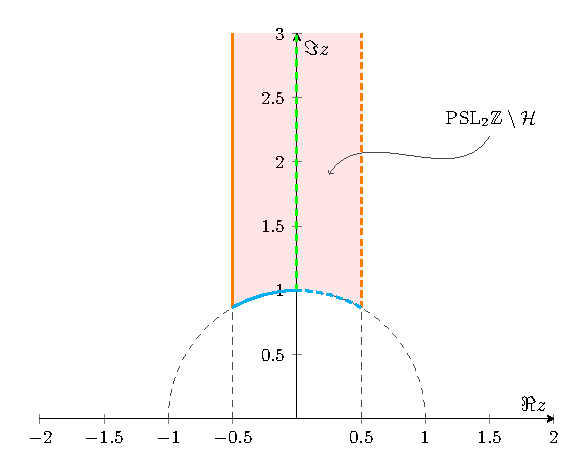
\includegraphics[scale=0.7,angle=0]{psl2.pdf}
  \noindent\\
  \decoRule
  \caption{Fundamental domain of modular surface.}
  \label{fig:fund_dom_psl2}
\end{figure}



At the link \url{https://roywilliams.github.io/play/js/sl2z/} it is possible to find a visualisation of point-orbits on the tassellation of the plane induced by $\PSL_{2}\Z$.

\begin{nese}[Bolza surface]
\label{ese:bolza_surface}
The \emph{modular surface} is the quotient $\Gamma\setminus\Hilb$ where $\Gamma=\PSL_{2}\Z$. The group $\PSL_{2}\Z$ is generated by the two matrices
\[
g_{k}=\Qmatrix{
1+\sqrt{2} & (2+\sqrt{2})\alpha\e^{\imi\frac{k\pi}{4}}\\
(2+\sqrt{2})\alpha\e^{-\imi\frac{k\pi}{4}} & 1+\sqrt{2}
},\quad\alpha=\sqrt{\sqrt{2}-1},\forall k=0,\ldots,7.
\]
\end{nese}

\begin{figure}[H]
\centering
  %
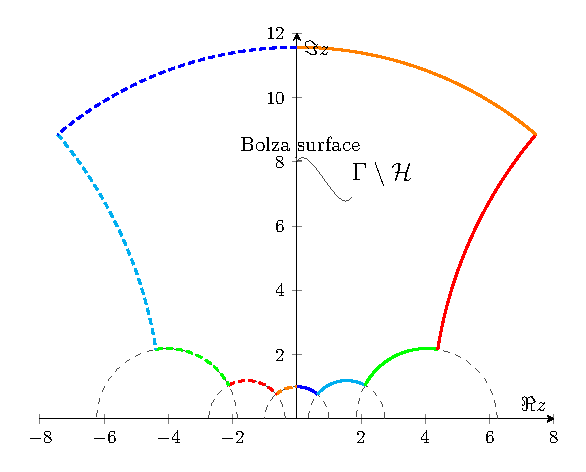
\includegraphics[scale=0.8,angle=0]{bolza_H.pdf}
  \noindent\\
  \decoRule
  \caption{Fundamental domain of bolza surface in $\Hilb$.}
  \label{fig:fund_dom_bolza_h}
\end{figure}

Considering the Dirichlet domain centered in $\Disk\ni z=0$, a fundamental domain for the Bolza surface is given by the hyperbolic octagon with vertices at point $2^{-1/4}\exp\left(\imi\left(\frac{\pi}{8}+\frac{k\pi}{4}\right)\right)$ for $k=0,\ldots,7$, with opposite sides identified.

\begin{figure}[H]
\centering
  %
  \begin{subfigure}[b]{0.4\textwidth}
  \centering
    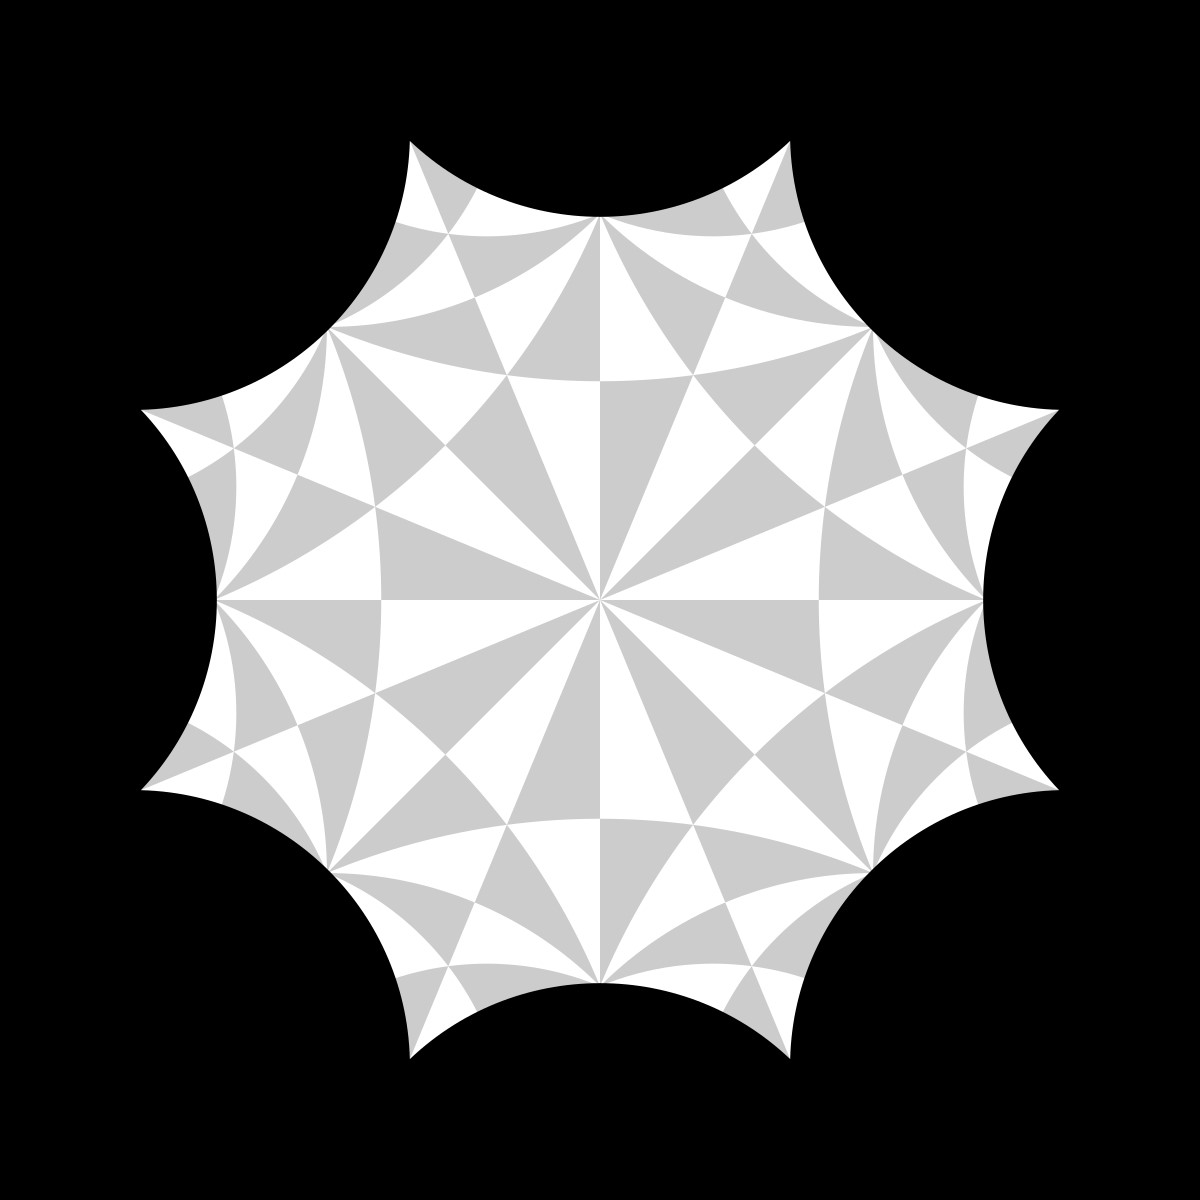
\includegraphics[scale=0.1,angle=0]{Bolza_cover238.jpg}
    %\caption{Variabili $X_{n}$}
    \label{fig:bolza_238}
  \end{subfigure}
  \begin{subfigure}[b]{0.36\textwidth}
  \centering
    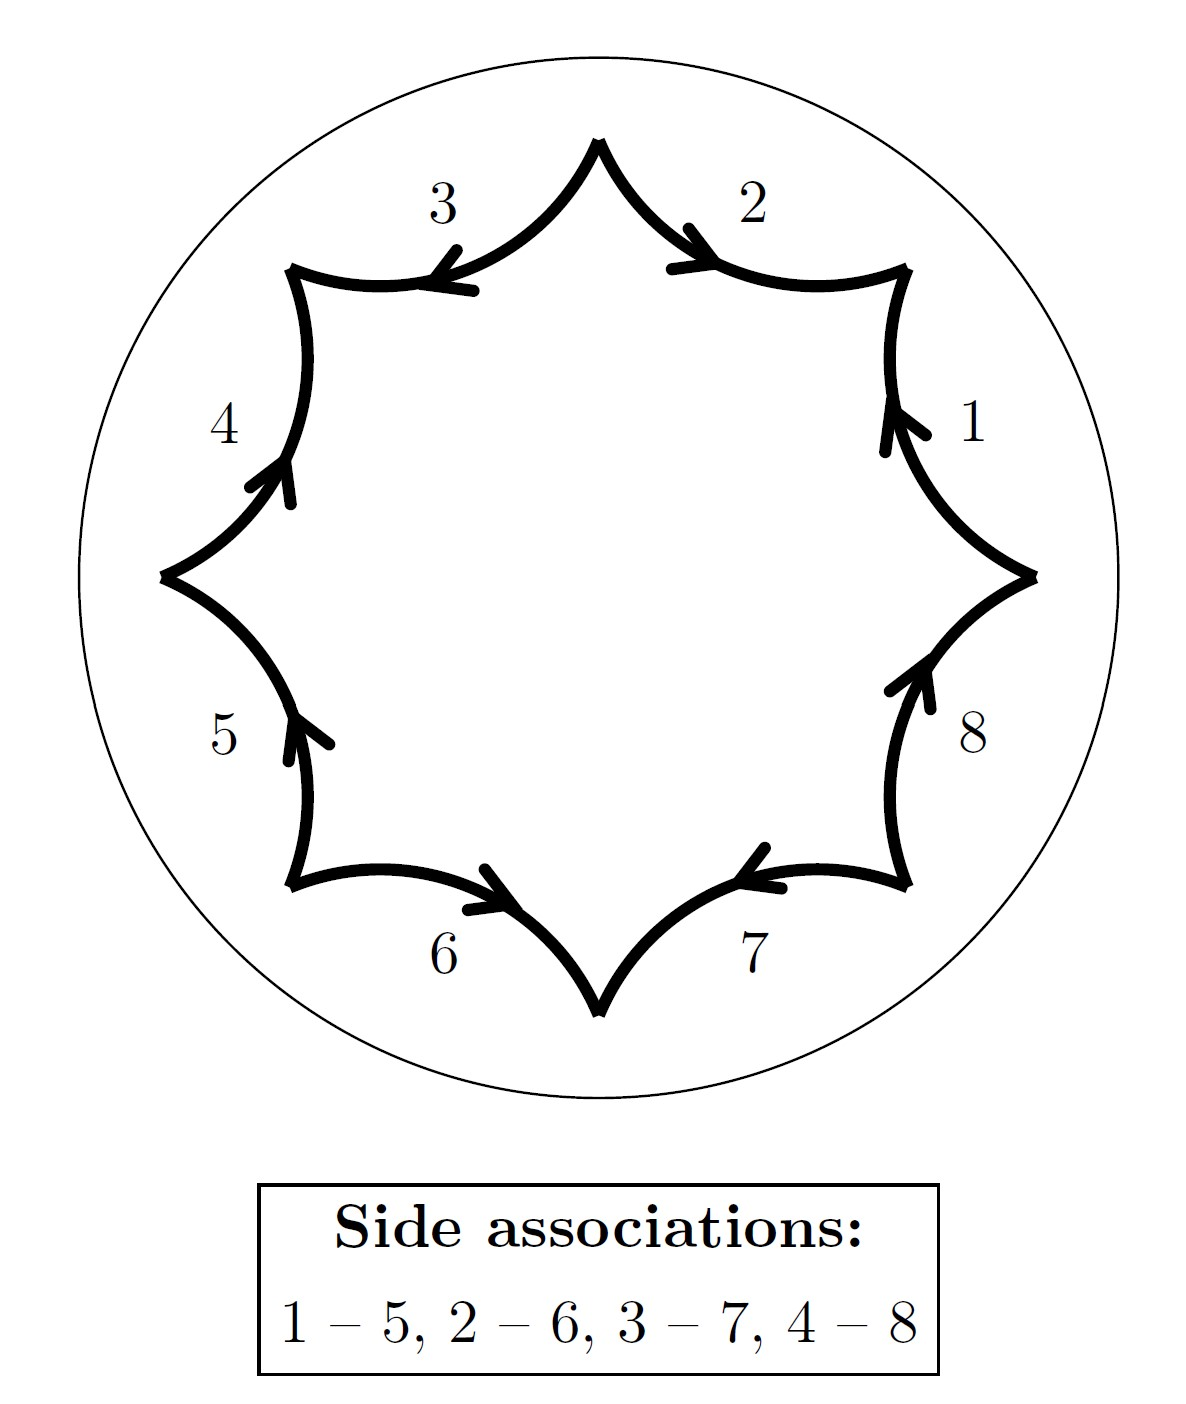
\includegraphics[scale=0.2,angle=0]{bolza_pair.jpg}
    %\caption{Variabili $X_{n}$}
    \label{fig:sides_bolza}
  \end{subfigure}
  \noindent\\
  \decoRule
  \caption{Bolza surface fundamental domain as subgroup of triangle group $\triang(2,3,8)$ (on the left) and with sides identification (on the right).}
  \label{fig:oval_card_orbits}
\end{figure}


There are two interesting facts about Fuchsian groups, which we will not prove (\cite{Katok:groups}).

\begin{defin}
\label{def:lattice}
A discrete subgroup $\Gamma<\PSL_{2}\R$ is a \emph{lattice} if it has a fundamental domain $D$ of finite area.
\end{defin}


\begin{nteo}[Siegel]
\label{teo:siegel}
If $\Gamma$ is a lattice, then any Dirichlet fundamental domain has finitely many sides.
\end{nteo}

\begin{nteo}
If $\Gamma$ is co-compact, i.e. the quotient $\Gamma\setminus\Hilb$ is compact, then $\Gamma$ has no parabolic element.
\end{nteo}

The rationale behind this result is that, is the quotient is compact, then it does not have point at extended real axis $\R\cup\{\infty\}$, so it cannot have parabolic elements whose fix elements lie on $\R\cup\{\infty\}$.








\section{Hyperbolic dynamics}


\label{sec:hyp_dynam}

\subsection{Geodesic flow}

The description given above can be regarded as a sort of \virg{discrete} motion induced by $A\in\PSL_{2}\R$ on a point of the unit tangent bundle $(z,\tau)\in T^{1}\Hilb$. So, the following question would be how to describe the continuos motion of a point $z$, given a direction $\tau$. This can be achived by the notion of \emph{geodesic flow}.

\begin{defin}
\label{def:geod_flow}
The \emph{geodesic flow} is a one parameter family of maps 
\[
a_{t}\colon T^{1}\Hilb\to T^{1}\Hilb
\]
for $t\in\R$, such that for any $(z,\tau)\in T^{1}\Hilb$ and $(\gamma(t),\gamma'(t))=a_{t}(z,\tau)$ is the unique geodesic parametrised by the \emph{arc length} satisfying $\gamma(0)=z,\gamma'(0)=\tau$.
\end{defin}

In the previous section, we have shown that, for each point $(z,\tau)$ there exist one and only and element $G\in\PSL_{2}\R$ such that $G(\imi,\imi)=(z,\tau)$, which is explicity given by equation \eqref{eq:main_matrix}. So the problem of parameterizing the geodesic starting from $z$ with direction $\tau$ can be brought back of parametrizing the geodesic starting from $\imi$ with direction $\imi$. However, we already now that this one is the vertical line $\imi t$ and an arc-length parametrization is given by $\imi\e^{t}$. In particular, we have that 
\begin{align*}
A_{t}(\imi,\imi)&=\Qmatrix{\exp(t/2)&\\&\exp(-t/2)}(\imi,\imi)\\
&=\left(\frac{\exp(t/2)\imi}{\exp(-t/2)},\frac{\imi}{(0+\exp(-t/2))^{2}}\right)=(\exp(t)\imi,\exp(t)\imi)
\end{align*}
which is the desired parametrization. Hence, for any $(z,\tau)\in T^{1}\Hilb$, if $G\in\PSL_{2}\R$ is such that $G(\imi,\imi)=(z,\tau)$, we have that
\[
a_{t}(z,\tau)=GA_{t}(\imi,\imi).
\]

In particular, recalling the Iwasawa decomposition \ref{impTeo:iwasawa}, via the identification of lemma \ref{lem:t1h_psl2_identification}, the geodesic flow is the right action of one parameter family 
\[
\Lie{A}=\left\{A_{t}=
\Qmatrix{\exp(t/2)&\\&\exp(-t/2)},\quad t\in\R
\right\}
\]
on the total group $\PSL_{2}\R$. There are other two fundamental flows on $T^{1}\Hilb$, corrisponding to different one parameter subgroups of $\PSL_{2}\R$. One is the (\emph{stable}) \emph{\textbf{horocycle flow}} by the one parameter subgroup
\[
\Lie{U}=\Lie{U}^{+}=\left\{
U_{t}=\Qmatrix{1&t\\&1},\quad t\in\R
\right\}
\]
and the other one is the \emph{unstable horocycle flow} given by 
\[
\Lie{U}^{-}=\left\{
U_{t}=\Qmatrix{1&\\t&1},\quad t\in\R
\right\}
\]
In figure \ref{fig:hyp_action_flows} it's possible to see the simultaneous action of the three groups on the point $(\imi,\e^{\imi\pi/3})$.

\begin{figure}[H]
\centering
  %
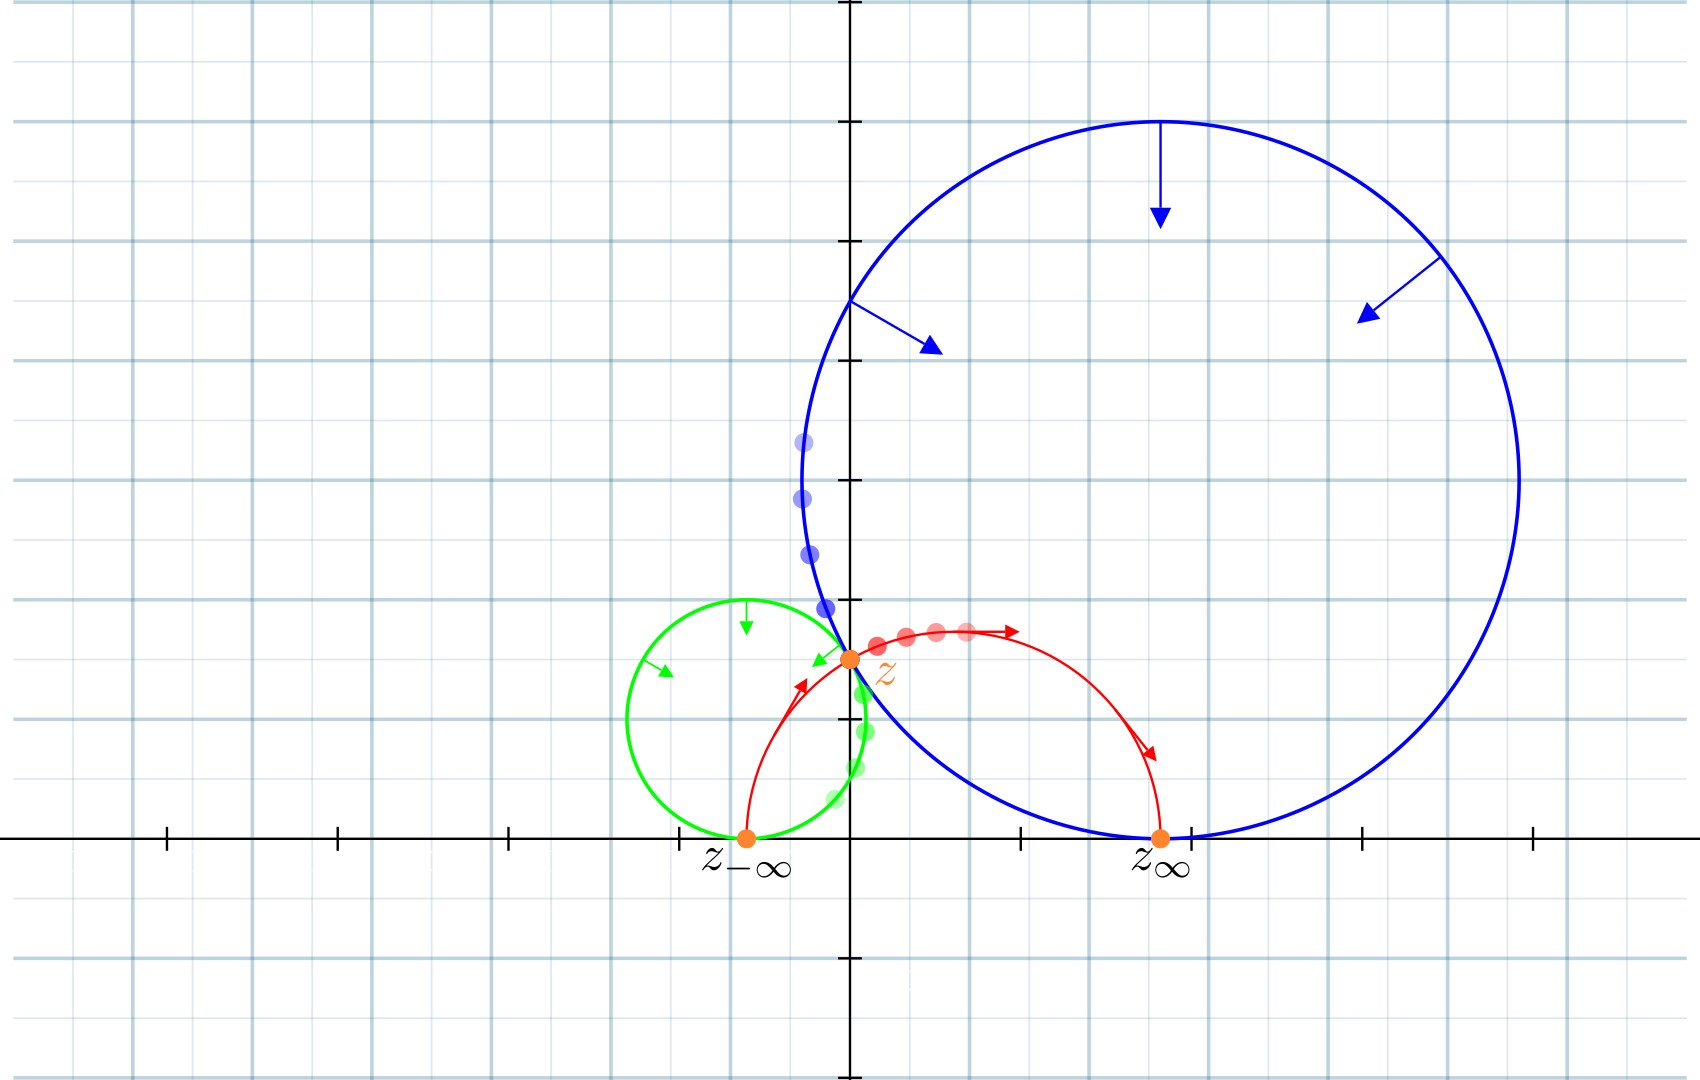
\includegraphics[scale=0.2,angle=0]{Flows.jpg}
  \noindent\\
  \decoRule
  \caption{Action of geodesic, stable and unstable horocycle flow.}
  \label{fig:hyp_action_flows}
\end{figure}



\subsection{Mixing flow on hyperbolic plane}

\label{subsec:mixing}

The area form on $\Hilb$ 
\[
\dd A=\frac{\dd x\wedge\dd y}{y^{2}}
\]
and the volume form on $T^{1}\Hilb\simeq\PSL_{2}\R$
\[
\dd V=\frac{\dd x\wedge\dd y\wedge\dd\theta}{y^{2}}
\]
are both invariant with respect to the action of the geodesic flow and horocycle flows, by virtue of theorem \ref{teo:area_volume_forms_invariants_isometries}, so it's interesting to study the corrisponding metric system.

We recall the notion of ergodic and mixing dynamical systems \ref{def:ergo_mix_continuos_system} (regarding the case of interest, we will use the continuos-case definitions). 

\begin{defin}
\label{def:ergo_mix_continuos_system}
Let $(X,\mathcal{X},\mu,R_{t})$ a continuos metric dynamical system (in particular $R_{t\ast}\mu=\mu\,\forall t\in\R$). Then:
\begin{itemize}
\item the flow $R_{t}$ is \emph{\boldsf{ergodic}} if for every measurable set $B\subset X$ which is $R_{t}$ invariant, $\mu(B)=0$ or $\mu(X\setminus B)=0$;
\item the flow $R_{t}$ is \emph{\boldsf{mixing}} if for every measurable sets $B,C\subset X$ 
\[
\mu(B\cap R_{t}^{-1}[C])\to\mu(B)\mu(C)
\]
holds, when $t\to\infty$.
\end{itemize} 
\end{defin}

These notions describes different manifestations of chaotich behaviour for a classical dynamical system. In particular, the mixing property is stronger than ergodic one: ergodicness of a system only assure that, in certain sense, that for a.e. point the orbit will go through all over the space $X$; on the other hand, mixing property regards how much a system \virg{mixes} itself. We will prove the following.

\begin{nteo}
\label{teo:geod_horo_are_mixing}
The geodesic and horocyclic flows are mixing.
\end{nteo}

This theorem is a direct consequence of a more general result about matrix coefficients of representations of subgroups of $\SL_{2}\R$. A unitary representation of a group $G$ on a Hilbert space $H$ is a group homomorphism
\[
\pi\colon G\to\U(H)
\]
where $U(H)$ denotes the group of unitary transformations. This representation is \emph{strongly continuos} if, for any $\vphi\in H$, the map $g\mapsto\pi(g)\vphi$ is continuos. 
\begin{defin}
Given $\vphi,\psi\in H$, the function $g\mapsto\pscl{\pi(g)\vphi}{\psi}$ is called a \emph{\textbf{matrix coefficient}} of the representation.
\end{defin}
In our situation, $\pi$ will be a representation of the group $G=\SL_{2}\R$ action on the Hilbert space $H=L_{2}(X)$ with $X=\Gamma\setminus G$, defined by 
\[
\pi(g)\vphi(h)=\vphi(gh),\quad\forall g\in G,\vphi\in L_{2}(X).
\]
In our context, the above definitions of ergodicity and mixing can be translated as follows.

\begin{defin}
Let $\Lie{U}_{t}$ be a one parameter subgroup of $\SL_{2}\R$.
\begin{compactitem}
\item The flow associated to $\Lie{U}_{t}$ is \emph{ergodic} if and only if for any $t\in\R$, $\pi(\Lie{U}_{t})$ has no non-trivial invariant vector.
\item The flow associated to $\Lie{U}_{t}$ is \emph{mixing} if and only if for any $\vphi,\psi\in L_{2}(X)$,
\[
\pscl{\pi(\Lie{U}_{t})\vphi}{\psi}\to \int_{X}\vphi\dd\mu\int_{X}\psi\dd\mu
\]
for $t\to\infty$.
\end{compactitem}
\end{defin}

The general result from which we will get the mixing of the geodesic flow is then.

\begin{impTeo}{Howe-Moore}{mixing_flow_psl2}
%\label{teo:mixing_flow_psl2}
Let $\pi$ be a strongly continuos unitary representation of $\SL_{2}\R$ on a Hilbert space $\Hilb$. Assume that $\pi$ has non-trivial invariant vector in $\Hilb$. Then, if $G_{n}$ is a diverging\footnote{That is for any compact $K\subset \SL_{2}\R$, there exists $N\in\N$ such that $G_{n}\not\in K$ for all $n\geq N$.} sequence in $\SL_{2}\R$, then 
\[
\lim_{n\to\infty}\pscl{\pi(G_{n})\vphi}{\psi}=\int_{X}\vphi\dd\mu\int_{X}\psi\dd\mu
\]
\end{impTeo}
\begin{prf}
See \ref{teo:mixing_flow_psl2_appendix}, in Appendix \ref{AppendixA}.
\end{prf}

In fact, in our case, the group $\SL_{2}\R$ acts transitively on $X$, so, if $f$ a invariant vector with respect to $\SL_{2}\R$, it must be constant, hence $\pi$ has no trivial invariant vector. The geodesic flow and the horocycle flow are given by the action of matrices $A_{t}$ and $U_{\pm t}$. In both cases, we are given a diverging sequence and so we are done.\\
\noindent\\
A mentioned in chapter \ref{Chapter1}, this is only a particular case of the more general result due to the Hopf, roughlt stated in \ref{teo:Hopf_theorem}.

\begin{impTeo}{Hopf}{hopf_ergodic}
%\ref{impTeo:hopf_ergodic}
Let $(M,g)$ be a compact Riemannian manifold with negative sectional curvature. Then the geodesic flow $\Phi_{t}\colon TM\to TM$ is ergodic.
\end{impTeo}


\subsection{Examples}


Although the geodesic flow on an hyperbolic surface is indeed ergodic, this does not prevent the existence of some periodic orbits. Nonetheless, these periodic orbits are very unstable, and little differences in initial condition produces very different behaviour during time evolution.



\begin{figure}[H]
\centering
  %
  \begin{subfigure}[b]{0.3\textwidth}
  \centering
    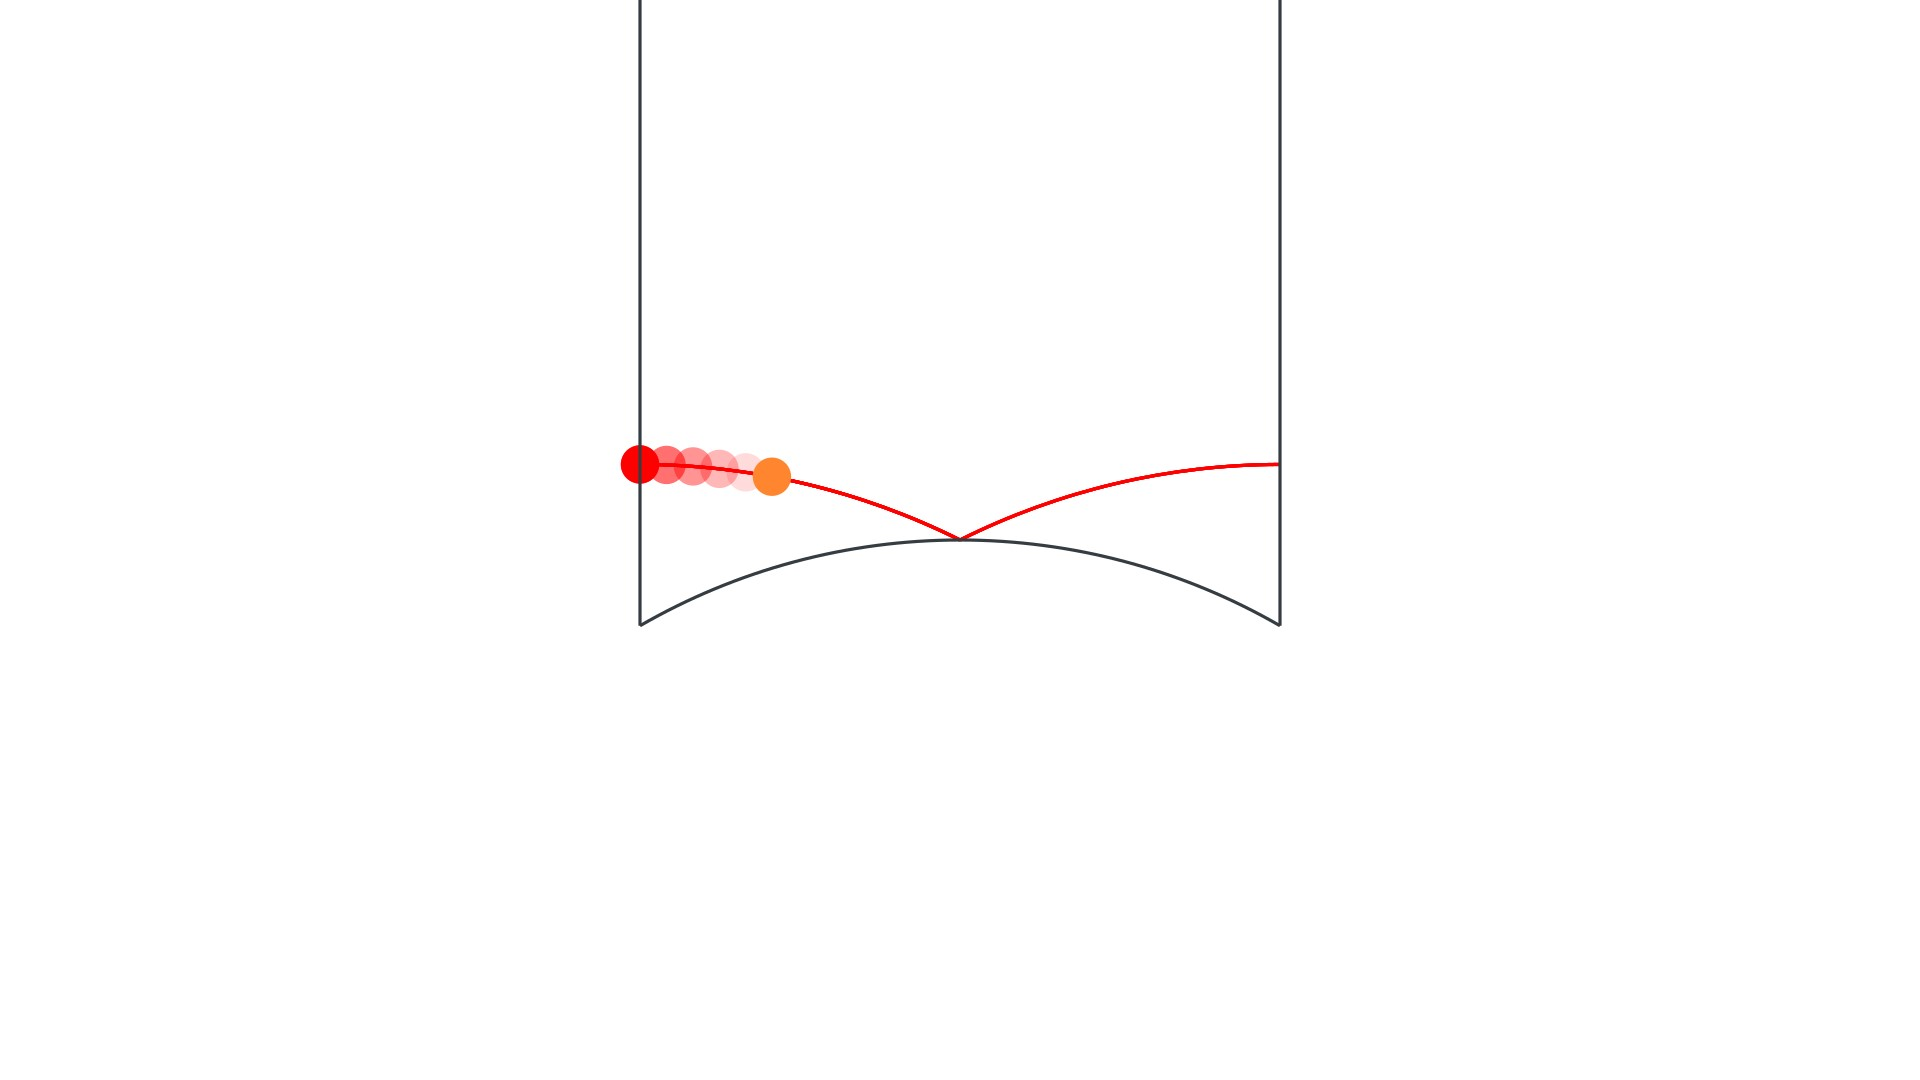
\includegraphics[scale=0.1,angle=0]{Periodic1.jpg}
    %\caption{Variabili $X_{n}$}
    \label{fig:mod_period_1}
  \end{subfigure}
  \begin{subfigure}[b]{0.3\textwidth}
  \centering
    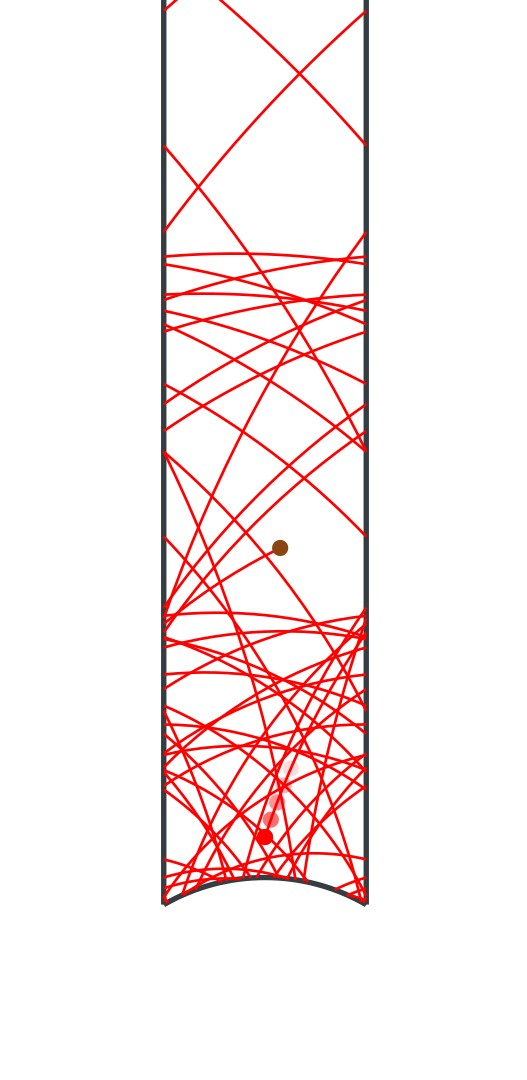
\includegraphics[scale=0.12,angle=0]{modular_billiard.jpg}
    %\caption{Variabili $X_{n}$}
    \label{fig:mod_erg}
  \end{subfigure}
    \begin{subfigure}[b]{0.3\textwidth}
  \centering
    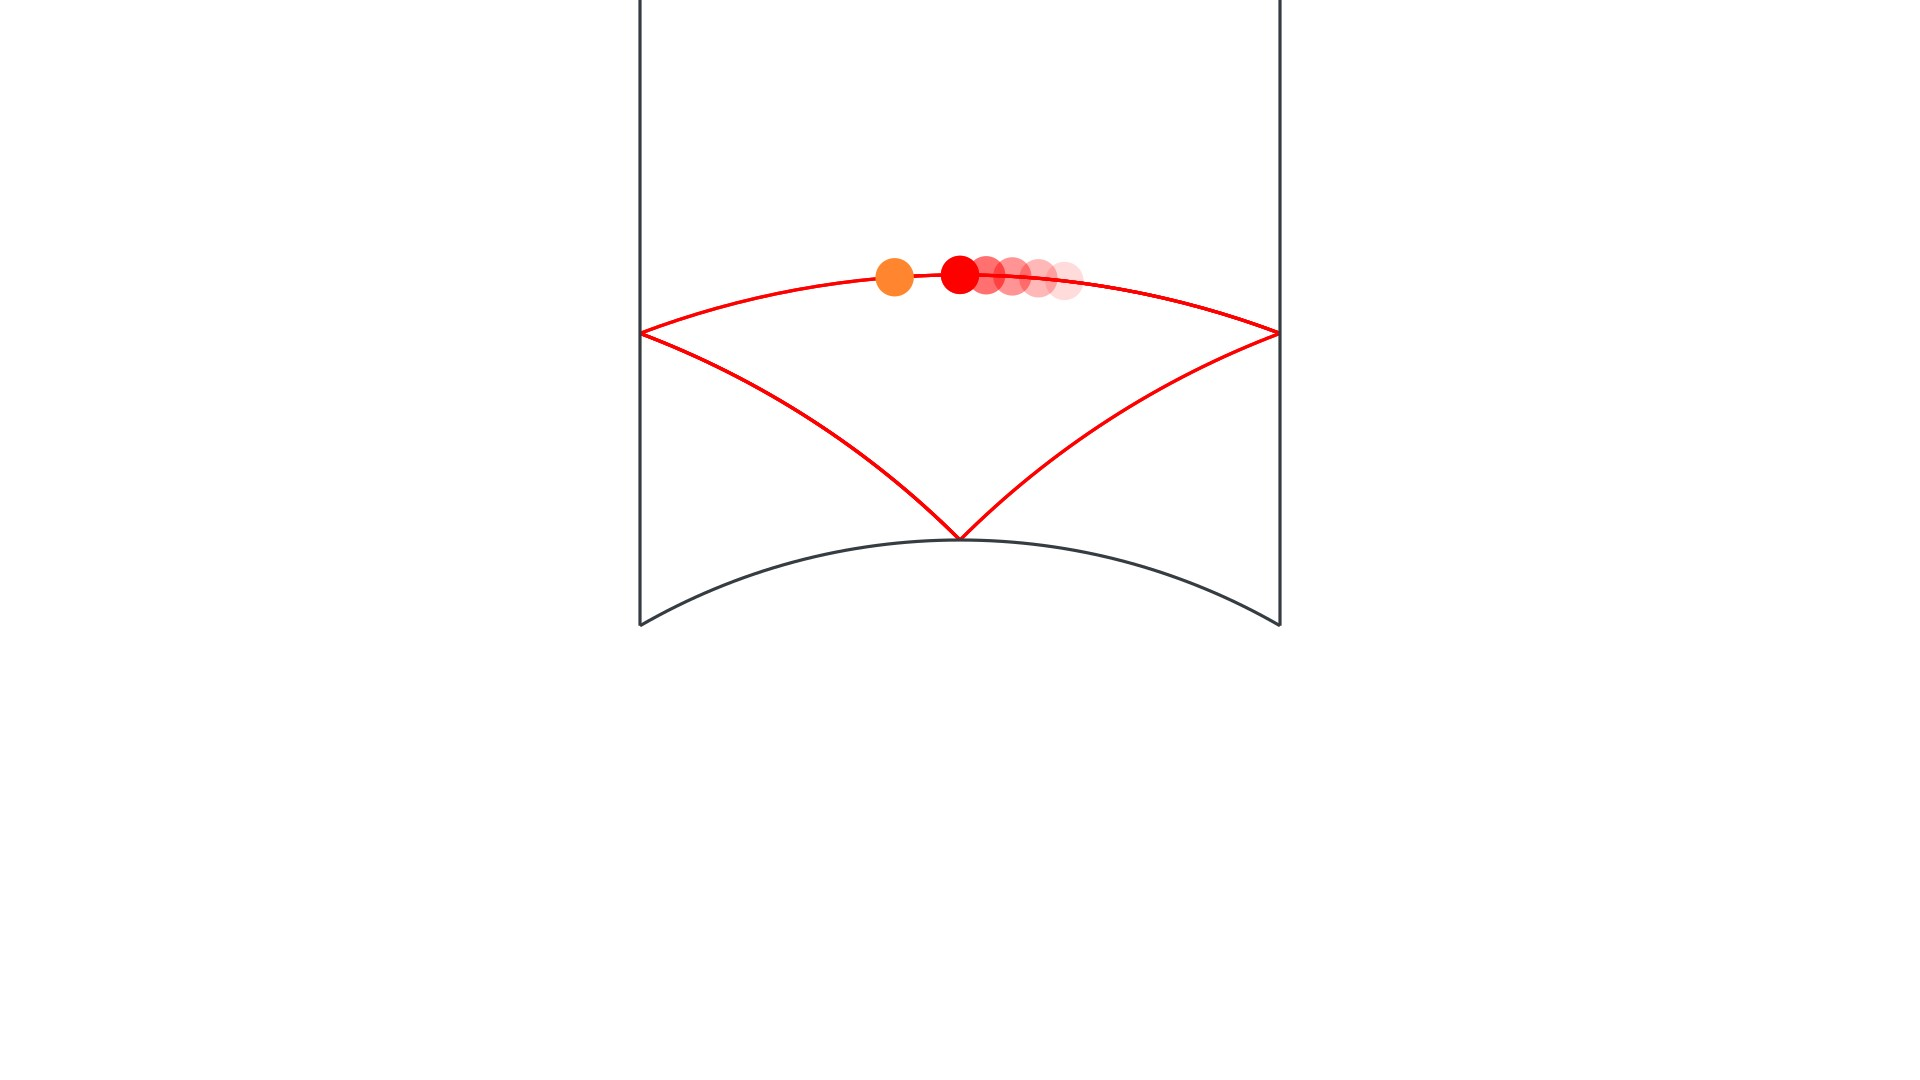
\includegraphics[scale=0.1,angle=0]{Periodic2.jpg}
    %\caption{Variabili $X_{n}$}
    \label{fig:mod_period_2}
  \end{subfigure}	
  \noindent\\
  \decoRule
  \caption{A typical chaotical orbit on the modular surface (in the center), along with two periodic orbits.}
  \label{fig:modular_orbits}
\end{figure}


As seen at the end of section \ref{subsec:hyp_isom}, hyperbolic elements $A\in\PSL_{2}\R$ have a fixed geodesic, which is its \emph{axis}. We can see periodic orbits on the modular surface as axis of particular hyperbolic elements, see also section \ref{sec:period_geodesics}. The two periodic orbits (of periods $4$ and $6$) in figure \ref{fig:modular_orbits} are given by the two matrices:
\begin{align*}
A_{l}=\frac{1}{2}\Qmatrix{5^{1/4}-5^{-1/4}&-(5^{1/4}-5^{-1/4})\\
2/5^{1/4}&2/5^{1/4}}&\colon\text{ figure on the left}\\
A_{r}=\frac{1}{6}\Qmatrix{3\sqrt{2}\sqrt[4]{3}&-3\sqrt{2}\sqrt[4]{3}\\
\sqrt{2}3^{3/4}&\sqrt{2}3^{3/4}}&\colon\text{ figure on the right}
\end{align*}


Using the \emph{Klein $j$-function}\footnote{DA SPIEGARE MEGLIO}, it is possible to visualize the above motions on the hyperbolic surface on the sphere, getting the images \ref{fig:modular_orbits_3d} (in it are visualized the periodic orbit of matrix $A_{r}$ and the above ergodic one).


\begin{figure}[H]
\centering
  %
  \begin{subfigure}[b]{0.3\textwidth}
  \centering
    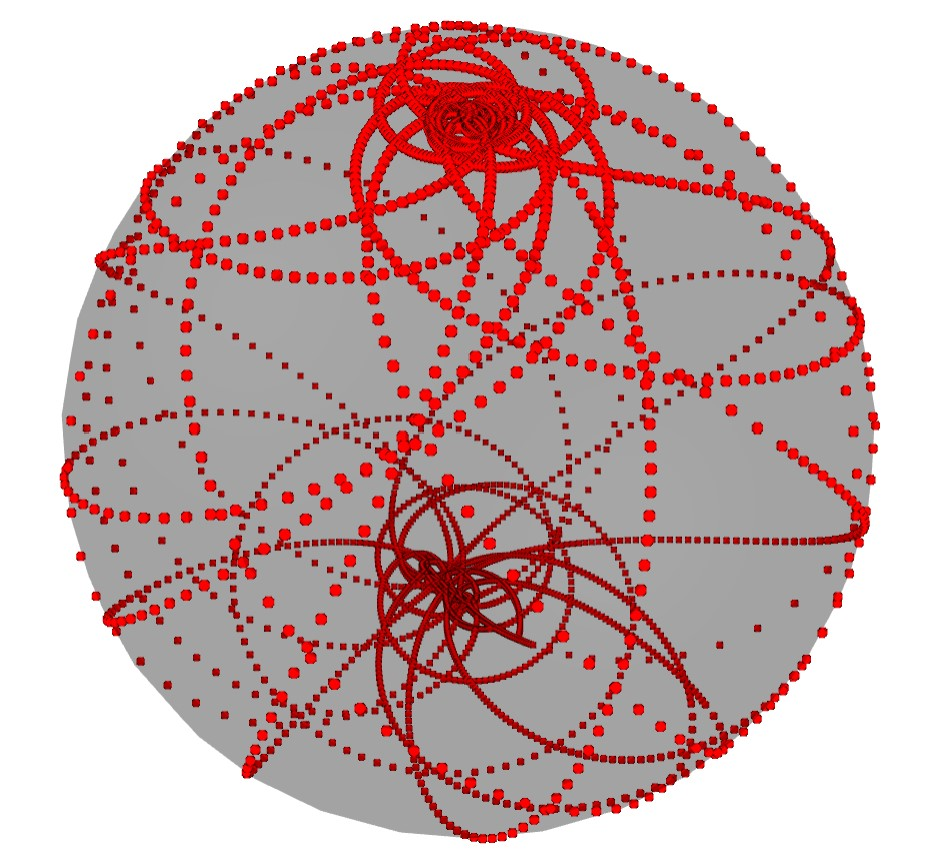
\includegraphics[scale=0.25,angle=0]{Orbit3D.jpg}
    %\caption{Variabili $X_{n}$}
    \label{fig:mod_3d_erg}
  \end{subfigure}
  \begin{subfigure}[b]{0.3\textwidth}
  \centering
    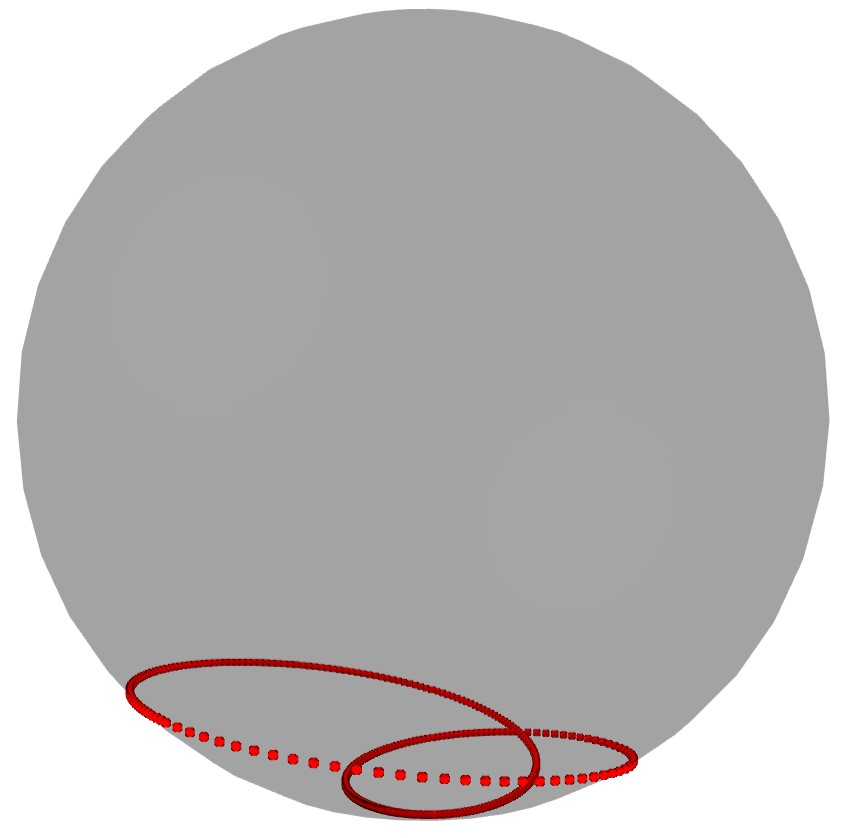
\includegraphics[scale=0.25,angle=0]{Orbit3Dperiod.jpg}
    %\caption{Variabili $X_{n}$}
    \label{fig:mod_3d_period}
  \end{subfigure}
  \noindent\\
  \decoRule
  \caption{3D visualisation of motion on hyperbolic surface.}
  \label{fig:modular_orbits_3d}
\end{figure}


%-----------------------------------
%	SUBSECTION 1
%-----------------------------------


%-----------------------------------
%	SUBSECTION 2
%-----------------------------------

%----------------------------------------------------------------------------------------
%	SECTION 2
%----------------------------------------------------------------------------------------

\section{Spectra of modular surfaces}

The modular group $\SL_{2}\Z$ has a particular importance in among the fuchsian groups, even if it (or better, its quotient $\PSL_{2}\Z$) can be seen just as a triangular group. This group has lots of arithmetic properties and for this reason it has been widely study, starting from its \emph{\textbf{principal congruence subgroups}} of level $N$ defined by
\begin{equation}
\label{eq:subgroups_congruence}
\Gamma(N)=\left\{
G\in\SL_{2}\colon G\equiv_{N}I
\right\}
\end{equation}
where the congruence \virg{$\equiv$} is taken componentwise. In general, a congruence subgroup of $\Gamma(1)=\SL_{2}\Z$ is a subgroup $\Gamma\leq\SL_{2}\Z$ for which there exists an $N$ such that $\Gamma\geq\Gamma(N)$ (roughly speaking, it is an \virg{upper subgroup of a principal congruence subgroup}).\\
The \emph{modular surface of level $N$} is then defined as
\begin{equation}
X(N)\coloneqq \Gamma(N)\setminus\Hilb.
\end{equation}
It is, for all $N\geq1$, a finite-area, non-compact hyperbolic surface. Just to emphasize the relevance of this subgroups, it can be shown that $X(1)$, with its complex structure, can parametrize the space of elliptic curves over $\mathbb{C}$, \cite{Shimura:book}.\\ %sanrak pg 3

Topologically speaking, the principal modular surface $X(1)$ is a like-sphere surface, with the hyperbolic metric and three \virg{cusp}. Moreover, its hyperbolic surface is equal\footnote{It is possible to use Gauss-Bonnet formula, which states that the hyperbolic area of a $\triang(a,b,c)$ is equal to $\pi(1-1/a-1/b-1c)$.} to $\pi/3$. To link the next chapter, we can now present the problem of our interest, which is the \virg{quantum-eigenvalue} problem

\begin{equation}
\label{eq:lapl_eingev_probl_hyp_surface}
\begin{cases}
\Lapl\vphi+\lambda\vphi&=0\\
\vphi(Gz)=\vphi(z)&;\forall G\in\Gamma\\
\int_{\Gamma\setminus\Hilb}\abs{\vphi}^{2}\dd\mu &<infty
\end{cases}
\end{equation}
with $\Gamma$ fuchsian group, in particular are extremly important the principal congruence subgroups $\Gamma(N)$. As we will see, the existence of a solution of the problem \ref{eq:lapl_eingev_probl_hyp_surface} is granted if the quotient space $X$ is compact, which is not the case for subgroups $X(N)$. This matter will be discussed in chapter \ref{Chapter6}. Avoiding the existence problem, solutions of problem \ref{eq:lapl_eingev_probl_hyp_surface} are called \emph{Maass forms}. 










